\section{Implementation} \label{design}

\subsection{Test setup and system design} \label{system design}

The central part of the game is based on the same setup and methods currently operated at CHBC. An initial meeting/brainstorming with CHBC was held to map out their expectation for a digitalized and automated version of their current methods. Furthermore, a hearing test was observed to see how their current methods would translate to a 3D game. 


\begin{figure}[h]
    \centering
    \includegraphics[width = 0.49\textwidth]{SMC2022_template_Latex/images/setup(2).jpeg}
    \caption{Testing setup for the automated CPA, based on the current setup at CHBC}
    \label{fig:setup}
\end{figure}

The first part of the design process was establishing a setup and test procedure for the new CPA, which matches the current methods and testing rooms at CHBC. The final setup can be seen in Figure \ref{fig:setup}. The child is placed in the middle of the room with a speaker and screen to the left, right, and front of the child. Two Azure Kinect in the corners are used to track the child's reaction to sound and to track gestures for controlling the game. As the game needs to be controlled precisely, also when the child is turned away from the Kinect, two Kinectsplaced at a 45$^{\circ}$ angle, should improve the skeleton tracking. The child is presented with an introduction from the front screen and speaker; afterward, the child is presented with a pure- or warble tone from either the left or right speaker. The Azure Kinect  tracks whether the child reacts correctly by looking toward the sound; if so, a fun and engaging game begins on the matching screen. The desired result is to engage the child in the test to play the game. When the game is over, the front speaker sends a message asking the child to look towards the front screen again so that a new tone can be presented.  \newline 

The design of the system was decided to be split into four different modules, which all will communicate with each other: 

\begin{enumerate}
    \item \textbf{Game-module: } This module contains all of the design (i.e., avatars and environment) and gameplay for the 3D game. This includes the design and methods for controlling the game. Furthermore, this module renders graphics on three different screens (see figure \ref{fig:setup}) . 
    \item \textbf{Kinect-module: } This module contains methods for accessing the data from the Azure Kinect to track the orientation of the child's head, the different gestures for controlling the game, and ensuring that the Kinect is following the correct body (i.e., if more than one person is in the room).
    \item \textbf{Sound-module: } This module contains methods for presenting pure- or warble tones at different frequencies and volumes (decibels) and methods for playing game sounds. This module must have access to specific outputs on the used audio interface to send sound to only the left, right or front speaker.
    \item \textbf{Control-module: } This module contains methods for changing the setup of the audio (i.e., mapping the different outputs of the audio interface) and the setup of the three different screens (i.e., what each display connected to the computer should render). Furthermore, the audiologist will use this module to control the loudness and frequency of the presented pure- or warble tones (i.e., by communicating with the Sound-module). All of this will be rendered on a separate screen, and whether the child reacted at the specific frequency and loudness will also be presented here. 
\end{enumerate}

\subsection{Game Design} \label{gameDesign}

The second part of the design process consisted of deciding on a game-play that worked well with the setup. From the initial brainstorming with CHBC, the idea of a Fruit Ninja\footnote{Fruit Ninja: https://www.halfbrick.com/games/fruit-ninja} inspired game was proposed. From the brainstorming, it was also deemed necessary that the child should be able to choose an avatar to personalize the experience. \newline

When beginning the hearing test, the child is presented with a scene in a temple with four different ninjas (see figure \ref{fig:ninjaAvatar}). 

\begin{figure}[h]
    \centering   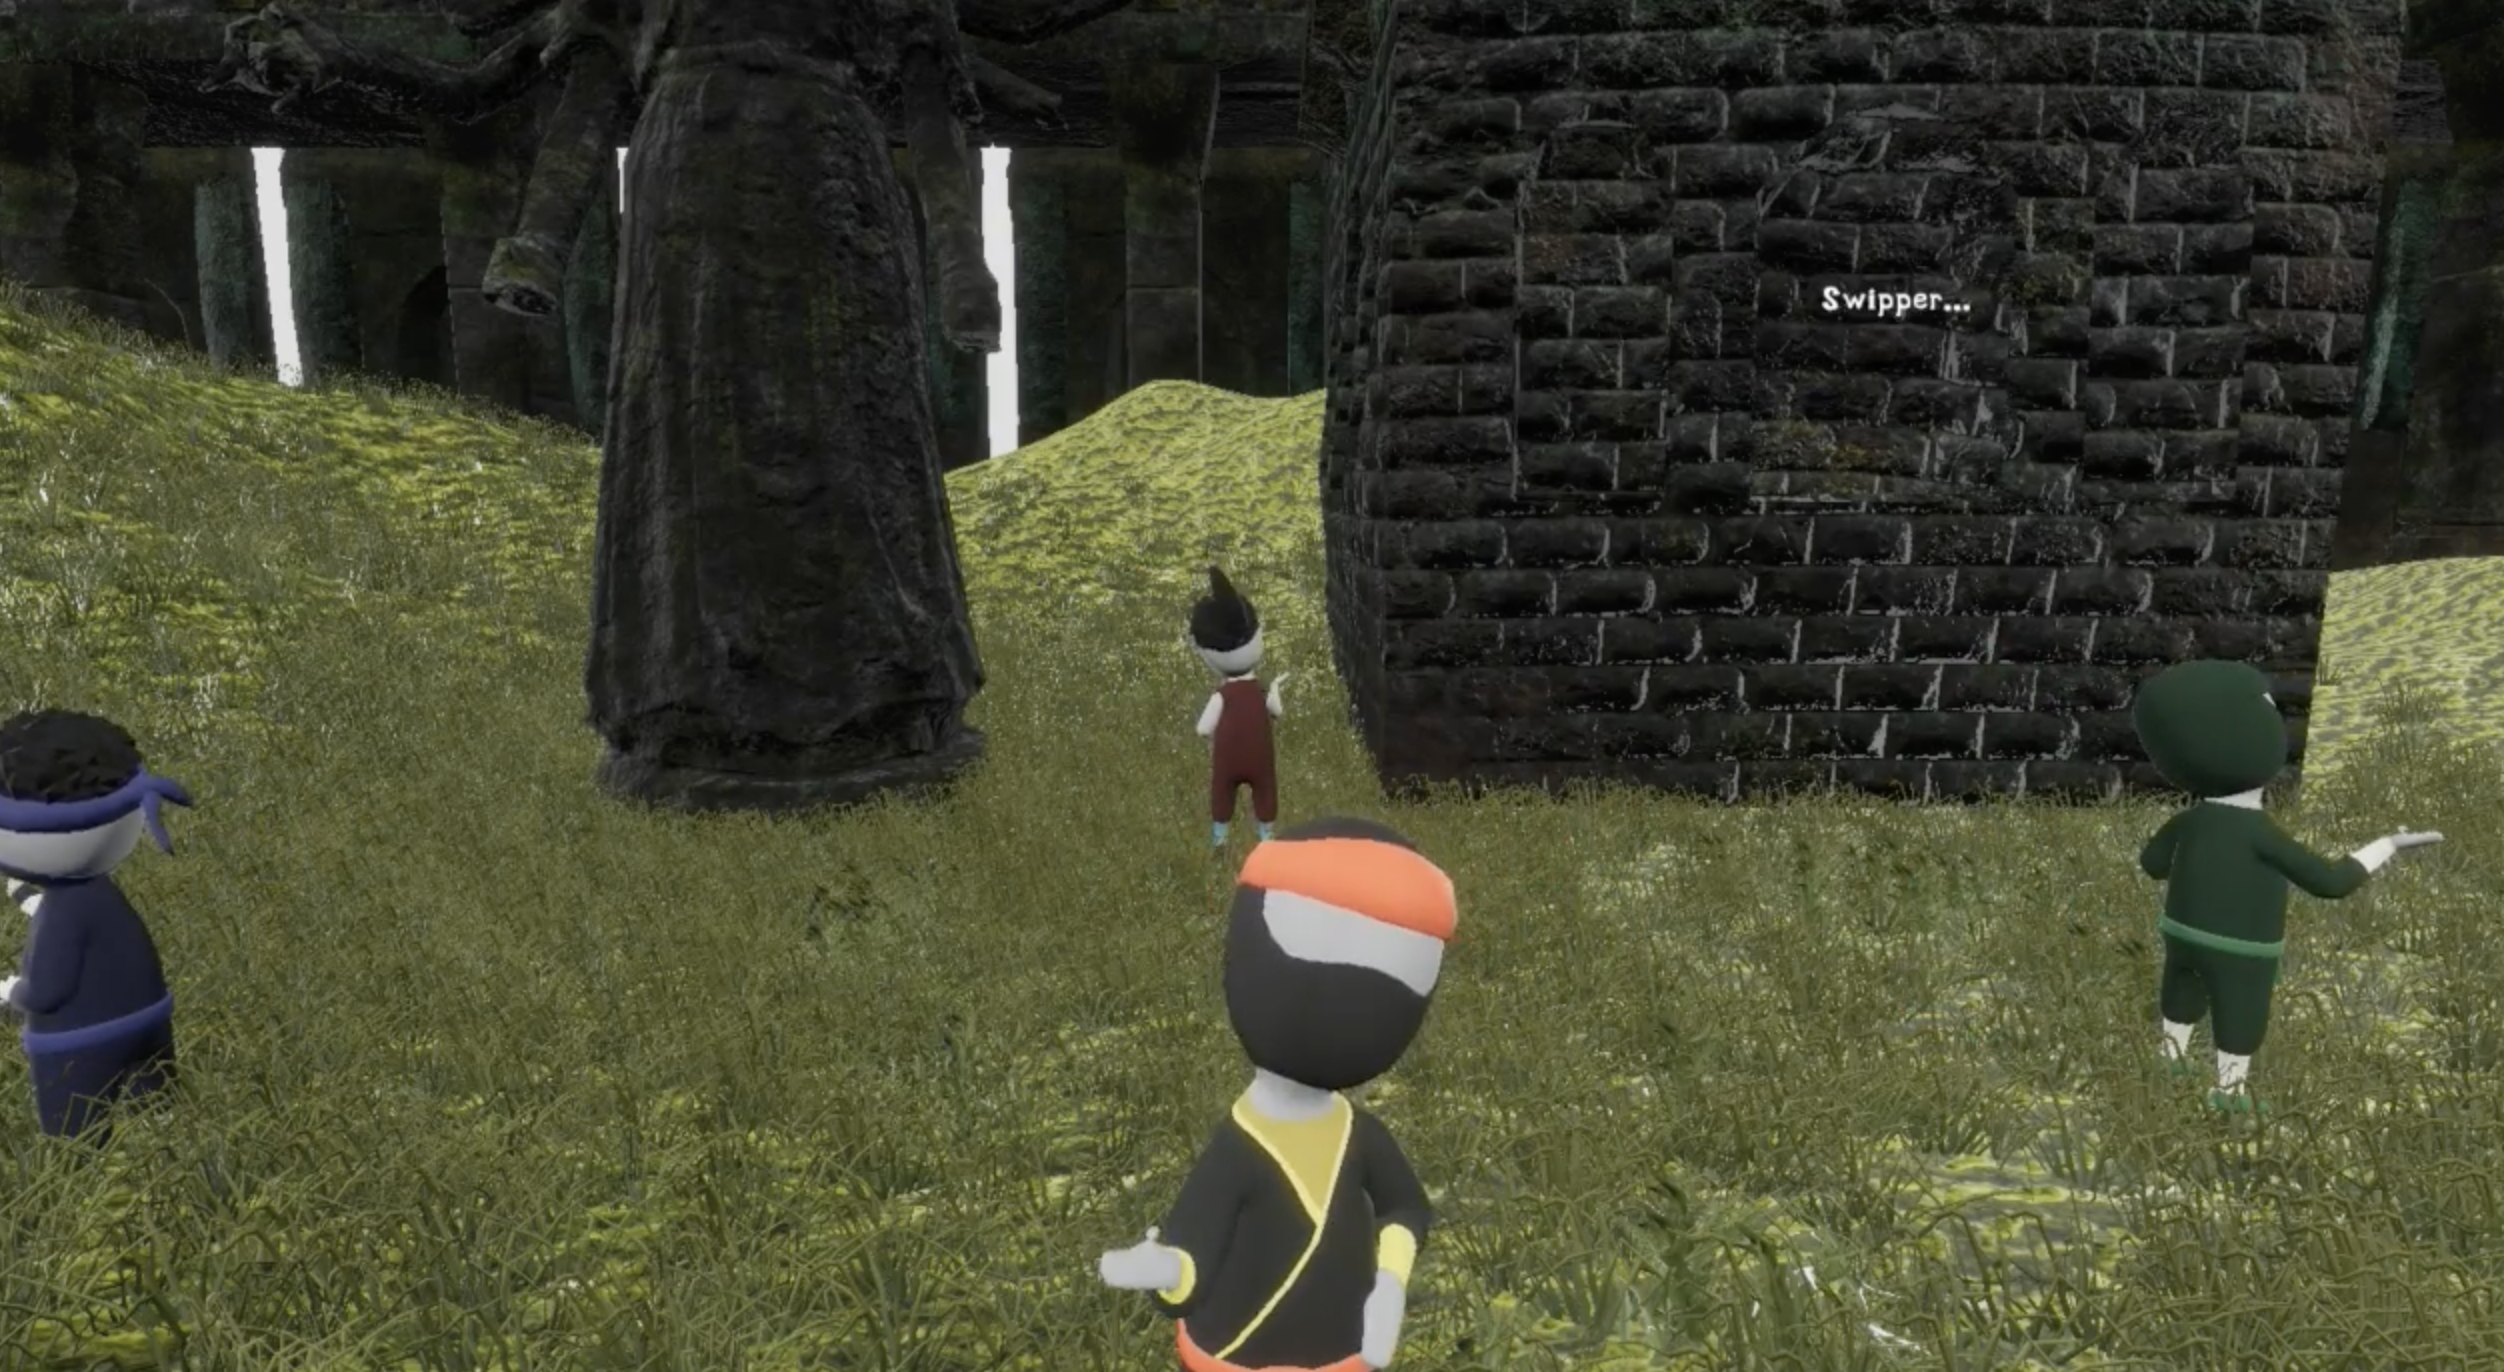
\includegraphics[width = 0.49\textwidth]{SMC2022_template_Latex/images/avatarchoose.png}
    \caption{Gameplay screenshot from the first scene in the game. The child can choose between four different ninjas by swiping.}
    \label{fig:ninjaAvatar}
\end{figure}

The child can choose a ninja by using a swiping gesture. When the child has found the preferred ninja, the child can start the hearing test by raising their left or right hand. After a small transition, the child will now see the 3D world from the chosen Ninja's point of view and can control the ninja with body movements. Another Ninja playing the role of a \textit{distractor} gives the child an introduction to the hearing test and asks the child to be quiet and look towards the sound when presented (see Figure \ref{fig:distractor}).

\begin{figure}[h]
    \centering   \includegraphics[width = 0.49\textwidth]{SMC2022_template_Latex/images/distractor.png}
    \caption{Gameplay screenshot from the introduction. An animated \textit{distractor} avatar introduces the child to the game.}
    \label{fig:distractor}
\end{figure}

The audiologist is now able to present a pure or warble tone, from either the left or right speaker, at a specific loudness and frequency, using the control-module (see figure \ref{fig:controlModule}). Before presenting a tone, the audiologist can choose an appropriate difficulty level for the child. The difficulty of the game ranges from 1 (easy, fruits coming slow, and are easy to hit) to 5 (hard, fruits coming fast, and are difficult to hit). 

\begin{figure}[h]
    \centering   \includegraphics[width = 0.3\textwidth]{SMC2022_template_Latex/images/playtone.png}
    \caption{Screenshot from the control module. The audiologist can play a pure- or warble tone at a specific frequency and loudness.}
    \label{fig:controlModule}
\end{figure}

After choosing randomly between 3 to 5 seconds from pressing \textit{play}, the tone is presented to the child.After playing the tone, the Kinect module detects  the child's reaction; if the child reacts correctly (i.e., looking towards the sound), a short Fruit Ninja-inspired game sequence will start on the matching screen (see Figure \ref{fig:fruitNinjaGame}). When done, the \textit{distractor} asks the ninja to look towards the front screen again, and a new tone is now ready to be presented. \newline

\begin{figure}[h]
    \centering   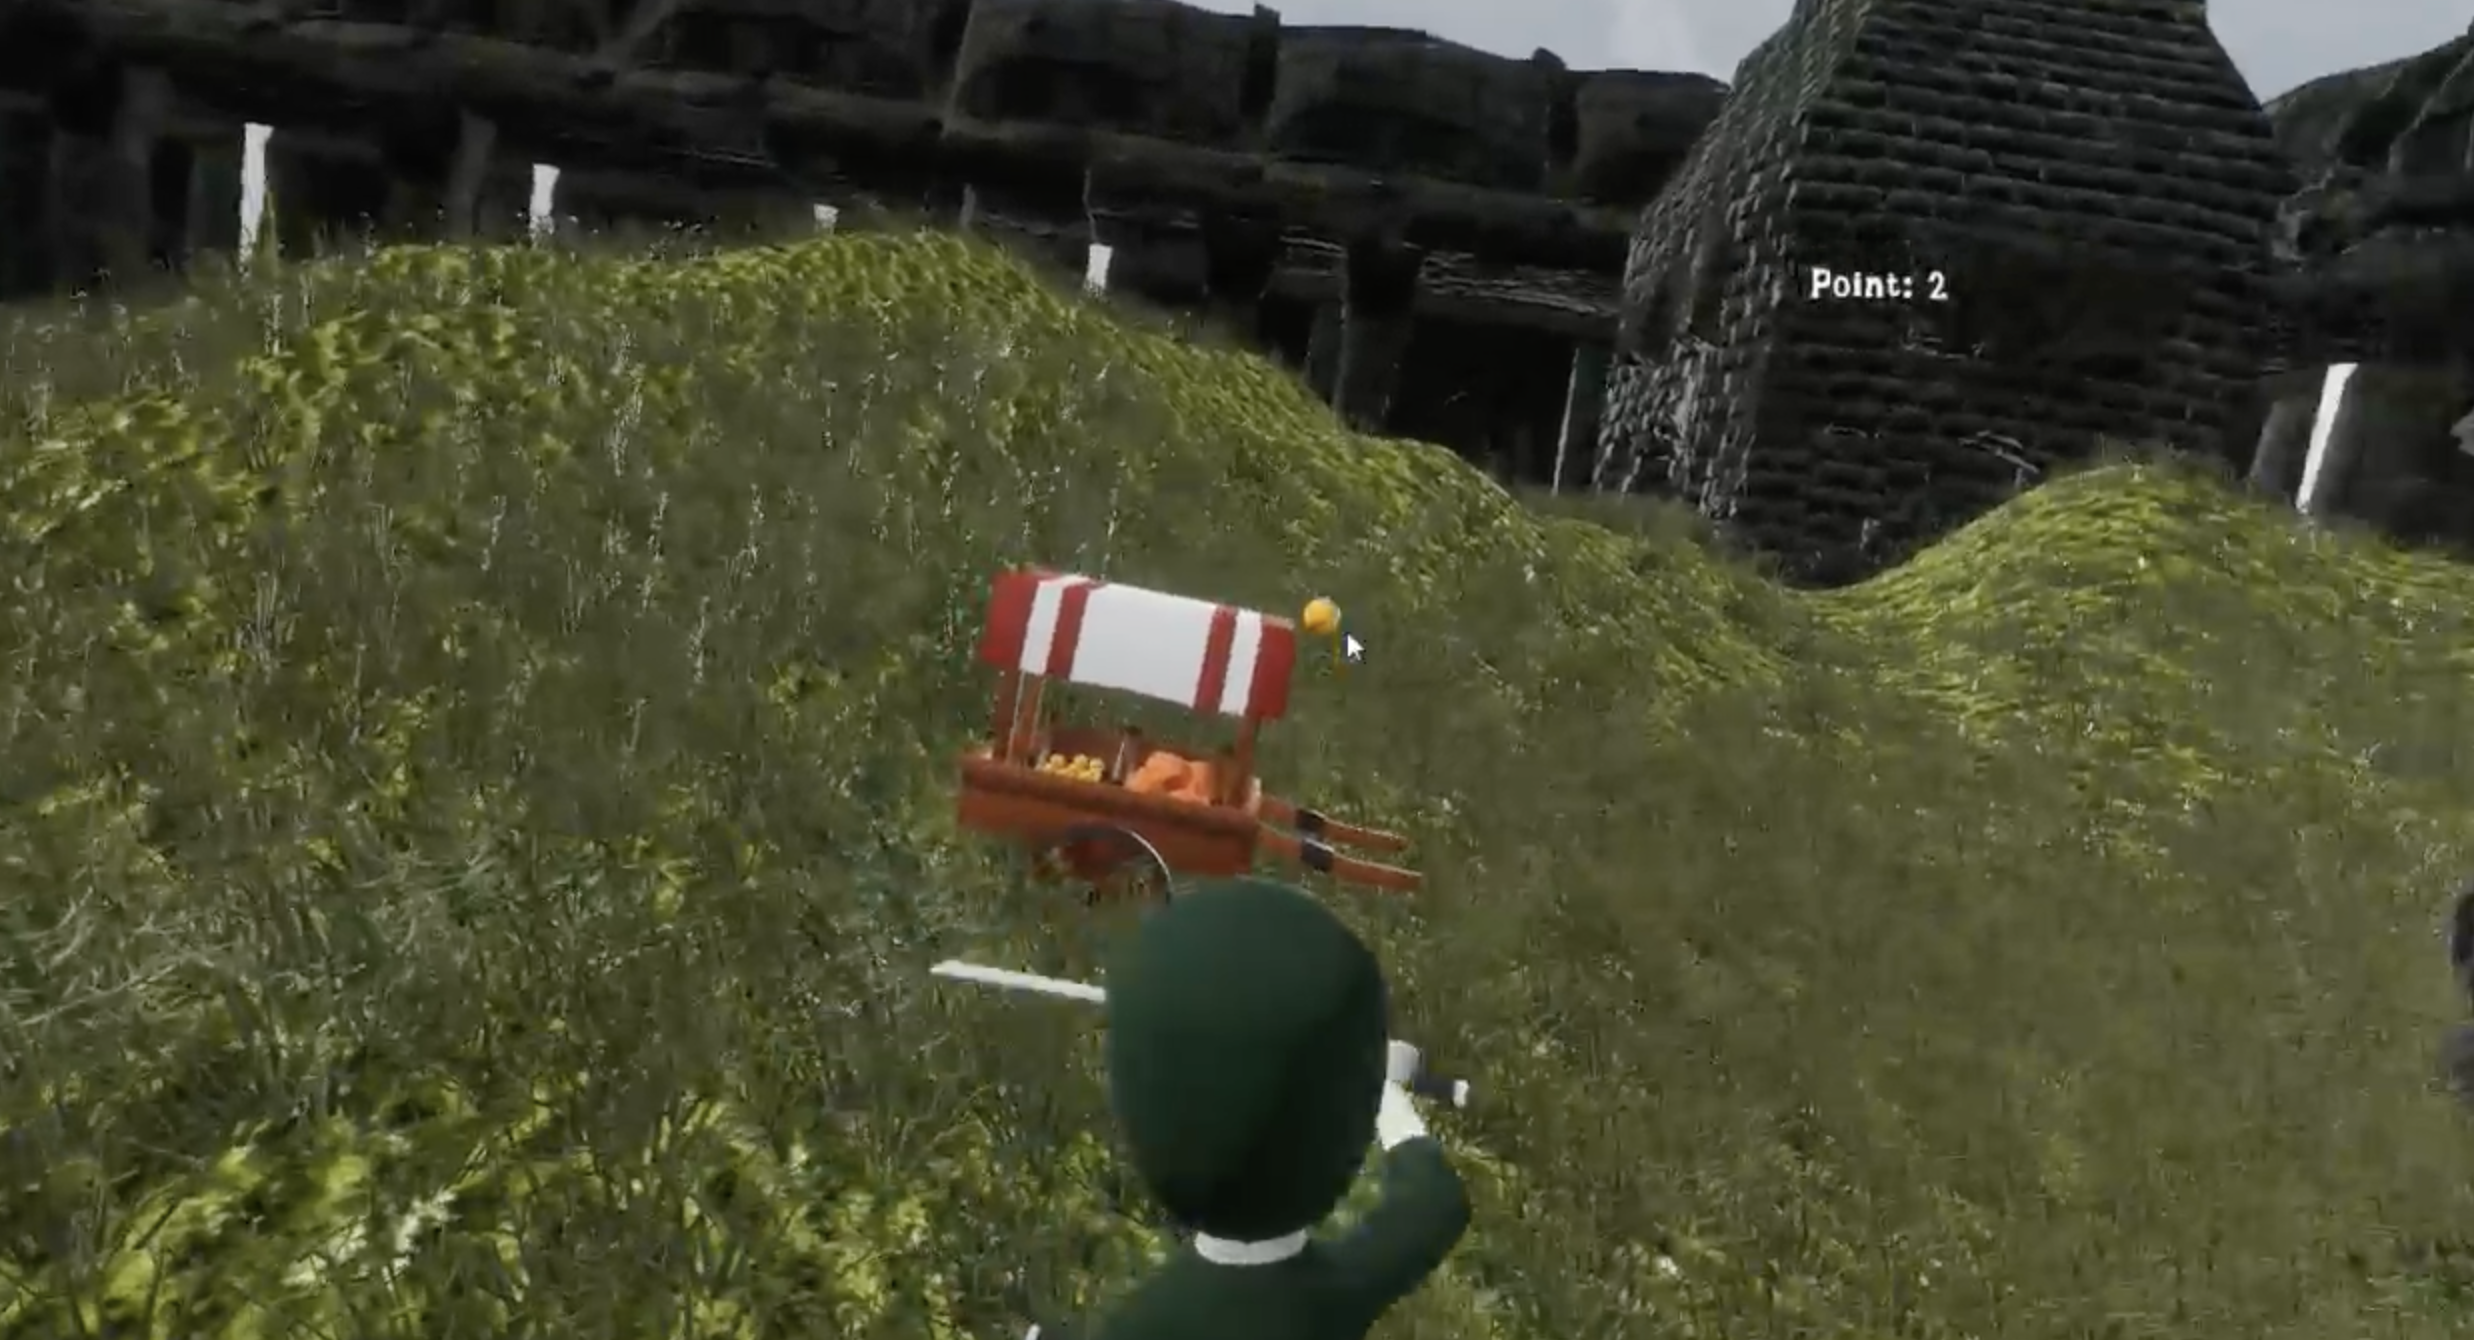
\includegraphics[width = 0.49\textwidth]{SMC2022_template_Latex/images/ingame.png}
    \caption{Gameplay screenshot from the fruit ninja game. The child can cut fruits and gain points by slicing fruits with their movements.}
    \label{fig:fruitNinjaGame}
\end{figure}


\subsection{Technical Description} \label{technicalDescription}
The prototype was designed and implemented using the
the Unity\footnote{https://unity.com/} game-engine.

\subsubsection{Azure Kinect Implementation}
For implementation of body tracking from the Azure Kinect, the Azure Kinect Examples for Unity\footnote{https://assetstore.unity.com/packages/tools/integration/azure-kinect-examples-for-unity-149700} package was utilized. The package includes methods for body tracking and for controlling avatars. The package also includes a Unity scene, which makes it easy to calibrate two Azure Kinects, which is needed for the setup presented in Section \ref{system design}. \newline

To ensure the Azure Kinect is tracking the correct body, a maximum and minimum distance on the z and x axis was implemented (see code in appendix \ref{appendix: UserTrackingCode}). The maximum and minimum distances are changeable from the control-module. 

\label{SoundImplementation}
\subsubsection{Audiometer implementation}

For the implementation of the play audiometer, the functional programming language Faust\footnote{https://faust.grame.fr/} was used. Faust has a wrapper system, which makes it easy to export the code to a real-time DSP to be used in Unity and be initiated at a specific frequency and loudness by the sound-module. Simple sine waves in the frequency range of 0.125 kHz to 8 kHz were implemented for the pure tone implementation. For the warble tone implementation, a frequency-modulated sine wave with a modulation rate of 5 Hz and a frequency deviation of 10\% was implemented (see section \ref{WarbleTones}). The modulation index is calculated as a ratio between the frequency deviation (in Hz) and the modulation rate (in Hz). This results in the following equation for the warble tone: 

\begin{equation}
    wt(f_{c},f_{m},f_{d}) = sin(2\pi f_{c}t+\frac{f_{c}f_{d}}{f_{m}}sin(2\pi f_{m}t)),
\end{equation}
\begin{footnotesize}
\textit{where $f_{c}$ is the center frequency in Hz, $f_{m}$ is the modulation rate in Hz and $f_{d}$ is the frequency deviation in percentages (e.g. 5\% frequency deviation is $f_{d} = 0.05$). }
\end{footnotesize} \newline


As the warble tone is generated in real-time by the Faust DSP in Unity, the frequency deviation and modulation rate is implemented to be changeable within the game controls in the control-module. As mentioned in section \ref{WarbleTones}, this give the possibility for the warble tone in the prototype to match any audiometer. The implementation in Faust code can be found in appendix \ref{appendix:faustCode}.


\subsubsection{Audio setup}

For the sound to work with the setup presented in section \ref{system design}, the sound-module must have access to specific outputs on a specific audio interface. As this functionality is not natively supported in Unity, the AudioStream\footnote{https://assetstore.unity.com/packages/tools/audio/audiostream-pcm-audio-for-unity-65411} package was utilized. The package includes methods for accessing all audio interfaces connected to the computer and channeling audio to specific audio outputs. All this is implemented to be controlled from the control-module to make the setup easy for any interface (see Figure \ref{fig:audioInterface}). 

\begin{figure}[h]
    \centering   
    \includegraphics[width = 0.49\textwidth]{SMC2022_template_Latex/images/14.12.2022_12.41.16_REC.png}
    \caption{Screenshot from the control-module. Utilizing AudioStream, it is possible to change the targeted audio interface and which output on the interface is the front, left, and right speaker.}
    \label{fig:audioInterface}
\end{figure}


